\documentclass{report}

\usepackage{graphicx}  % поддержка .eps-графики
\usepackage[utf8]{inputenc} % кодировка в которой набран текст 
\usepackage[T2A]{fontenc} % поддержка кирилицы % ещё можно T1 T2B
\usepackage[english,russian]{babel} % переносы и типографские правила для русского
\usepackage{indentfirst}  % красная строка
\usepackage{listings}  % оформление листингов программ
\usepackage{amssymb,amsfonts,amsmath,mathtext} % ядро для научной статьи
\usepackage{physics}
\usepackage{mathtools}
\usepackage{braket}
\usepackage{float}

\graphicspath{{./images/}} %путь к рисункам
\frenchspacing % длина пробелов после пунктуации
\pagestyle{plain}

\begin{document}

\title{Как писать научные статьи}
\author{Mark Zaslavskiy}
%\institute{Донской Государственный Технический Университет}
\date{\today}
\maketitle
\tableofcontents
\newpage



\section*{Описание курса}

На сегодняшний день написание научных статей перестало быть уделом только ученых. Современные образовательные стандарты подразумевают подготовку научных публикаций в течение обучения в бакалавриате и магистратуре. При этом начинающим авторам бывает сложно подготовить свою первую статью, так как навык написания научных работ требует широкого объема знаний и умений, которые, зачастую, не преподаются целенаправленно. Цель курса - дать целостное введение в подготовку текста научной статьи.

Из материалов курса вы узнаете ответы на следующие вопросы:

Что такое научная статья и в чем заключается научность?
Какая структура должна быть у научной статьи?
Как найти аналоги даже если кажется, что их нет?
Как подготовить черновик статьи?
Что такое научный стиль письма и как им овладеть?
Как выбрать издание и подать статью к публикации?
Как реагировать на результаты рецензирования и добиться публикации вашей статьи?
Материалы курса сформулированы на основании опыта научных публикаций в отечественных и зарубежных научных журналах, а также выступлений на международных научных конференциях.

\chapter{Введение}

\section{Что такое научная статья и зачем она нужна}
Что такое научная статья?
Научная статья - это краткое изложение результатов научного исследования, опубликованное в научном издании. При этом исследование может быть как авторским, так и исследованием (сравнением, обобщением) работ других ученых.
Помимо изложения результатов научного исследования статья обладает следующими признаками:

\begin{enumerate}
	\item Обоснованность - предлагаемые утверждения доказаны формально или иным, принятым в научном сообществе способом.
	\item Формальная постановка - в работе присутствует максимально точная и емкая формулировка решаемой задачи.
	\item Соответствие формату - работа соответствует общепринятым требованиям к стилю написания и оформления научного текста.
	\item Научность результатов, о которой будет сказано далее.
\end{enumerate}

Ваша цель в том, чтобы превратить результаты вашего исследования в опубликованную работу.

\begin{figure}[H]
\centering

\includegraphics[width=13cm]{main_sheme}
\caption{Общая схема подготовки научной статьи.}
\end{figure}


\subsection{О научности}

Научность каких либо результатов исследований, научность работы, и определение науки являются сложными понятиями.

В курсе предложена упрощенная модель научности статьи, которая поможет подготовить первую научную статью.

Предлагаемая модель необходима, чтобы писать статьи начального уровня по техническим специальностям, и основывается примерно поровну на философии науки 20 века и на личном опыте научных публикаций авторов курса.

Для того чтобы считать статью научной, необходимо, чтобы ее содержание соответствовало пяти критериям:


\begin{itemize}
	\item проблемная ориентированность
	\item критерий развития
	\item верифицируемость
	\item связь с работами других ученых
	\item критикуемость
\end{itemize}

Самым важным критерием научности является проблемная ориентированность. Ваша работа (статья) должна быть связана с какой-то проблемой: технической, научной, научно технической или общечеловеческой.

Важно в статье был предмет и она была каким-то шагом в решении определенной проблемы. Если этого нет, то это можно назвать размышлениями на тему, но назвать это статье уже достаточно сложно. В статье начального уровня должно быть четкое позиционирование какой-то проблемы и, попытка если не решите ее, то как-то подкопаться к ее решению. Соответственно, отсюда вытекает критерий развития.

Критерий развития - это какая-то явная или неявная польза от вашей статьи. Если есть какая-то проблема и по ней пишется научная статья, важно чтобы ваша статья как минимум продвинула научное знание. В любом случае, ваша статья должна обладать некоторой значимостью и приносить какую-то пользу научному сообществу, техническому сообществу или давать вообще какой-то глобальной эффект.

Критикуемость. Для вашего текста, для вашей научной работы, для ваших результатов всегда должно оставаться пространство для конструктивной критики другими учеными. Переходя на терминологию программистов, серебряной пули не существует, если ваша работа выглядит как серебряная пуля, то это вызывает очень сильное желание читателей, рецензентов или редакторов вашу работу атаковать. Если вы изобрели какую-то свою теорию взаимодействия или свою теорию гравитации, которая абсолютно непротиворечива и к ней никак не подкопаться. Или если вы изобрели абсолютный алгоритм распознавания чего-либо, которой работает идеально, не потребляет памяти, работает за мгновенно, то подумайте, может быть, у него есть какие-то слабые стороны, недостатки которые оставляют вашим читателям пространство для критики. Отсюда следует связь с работами других ученых.

Связь с работами других ученых. Наука развивается постепенно. Новый результат так или иначе всегда базируется на результатах ученых, которые были до вас. Например: если вы занимаетесь небесной механикой, вы так или иначе опираетесь на труды физиков, которые были до вас.

\begin{itemize}
	\item Птолемей: все небесные тела вращаются вокруг центра - Земли.
	\item Коперник: другое тело находится в центре - Солнце
	\item Кеплер - орбиты немножко другие. То есть, развитие науки поступательно и постепенно, и, если вы предлагаете какой-то новый результат, какие-то ваши исследования приносят новые знания, это должно быть связано с работами других ученых. Должно опираться на их плечи и быть привязано к существующему формализму или быть связано с существующими моделями и подходами, принятыми в данной науке. Поэтому, если вы предлагаете теорию гравитации, которая уникальна и абсолютно никак не связана с Ньютоном или Эйнштейном, то это повод задуматься над научности вашей работы.

\end{itemize}

Верифицируемость. Ваши результаты должны быть проверяемые и повторимы. Наука зиждется на доказательности. Например, никто не будет запускать в оборот лекарство без испытаний на животных. Когда это требование выполняется и как это понять? Например, если вы изобрели какой-нибудь хитрый вечный двигатель, но для его работы требуется какие-то совершенно не воспроизводимые на Земле условия, например, условиях первых секунд секунд после Большого взрыва или внутренности черных дыр. Должно быть, что он будет работать, но только вот в этих условиях, и никто не может проверить, никто не может даже попытаться как-то верифицировать ваши результаты. В этом очень слабое место вашей работы и в этом нарушается ее научность. Результаты ваших исследований должны быть сформулированы таким образом, чтобы другие ученые могли как минимум оценить или проверить ваши слова. В лучшем случае должна присутствовать процедура проверки или она должна быть очевидна из того что вы предлагаете.

\subsubsection{Оговорка про критерии научности}

Необходимо понимать, что восприятие вашей статьи зависит не столько от глубины проделанного вами исследования, сколько от качества его описания и презентации в статье. Если вы проделали хорошее исследование, но плохо его описали, то с высокой вероятностью его не опубликуют.

Для успешной публикации, критерии научности должны выполняться как для содержания вашего исследования, так и для текста самой статьи.

\subsubsection{Позиционирование относительно работ других ученых}
Позиционирование относительно работ других ученых
Для того, чтобы научность вашей работы не вызывала сомнений, необходимо однозначно ответить для себя и отразить в тексте, как ваша работа связана с существующими научными результатами. Ниже мы представили несколько типовых вариантов.

Наиболее частым способом позиционирования является расширение и/или улучшение существующей модели. Примером может служить расширение ньютоновской физики в теории относительности (ТО). Для малых скоростей и масс формулы ТО сводятся к формулам классической механики.

Если вы не предлагаете новых моделей, то ваше позиционирование относительно работ других ученых может выглядеть как восполнение исследовательских пробелов (дополнительные эксперименты, уточнение/оценка коэффициентов и т.д.) для существующих моделей, либо как их новое практическое применение (оценка эффективности работы обобщенных алгоритмов сжатия изображений на фото птиц).

Однако, даже в случае, когда предыдущие варианты не работают и ваши результаты выглядят действительно новаторскими, все равно существует связь между вашей работой и трудами классиков. Этой связью будет использование устоявшихся терминов, обозначений и понятий.

Даже в случае, если вы полностью перечеркиваете предыдущие результаты других исследователей своими блестящими построениями, вам будет необходимо продемонстрировать ошибочность старых представлений о проблеме.

\subsubsection{Ссылки}
С технической точки зрения опора на других ученых реализуется  с помощью механизма ссылок. В каждой научной статье есть такой раздел как "Список литературы". Он может также называться:

Литература,
Список использованных источников,
References.
В данном разделе перечисляются основные источники, на которые опирался автор статьи. Как правило, факт опоры оформляется в тексте в виде указания номера источника из списка в квадратных скобках, однако встречаются и другие способы оформления.

При цитировании важно понимать, что научность вашей работы (в частности выполнение критерия "Опора на других ученых") напрямую зависит от списка литературы и корректности цитирования и расстановки ссылок. Ссылки на сомнительные или не авторитетные статьи с высокой вероятностью вызовут у редактора сомнения в вашей научной квалификации.

Поэтому, необходимо придерживаться следующих рекомендаций:

Читайте источники перед добавлением в список литературы.
Каждый источник из списка литературы должен иметь минимум одну ссылку в тексте.
Ссылайтесь на статьи и книги, чей авторитет является общепризнанным. Как правило, такие издания являются фундаментальными трудами в вашей области, а статьи - наиболее цитируемыми.
Данные рекомендации могут пока показаться довольно туманными, однако даже на текущем этапе вы можете начать сбор источников в список, часть из которого перекочует в вашу статью.

\subsection{С чем путают научную статью}

Мы поняли, что такое научная статья, мы понял, каким критериям нужно соответствовать и примерно что статья собой представляет. Хочется рассказать об одном важном моменте. У начинающих авторов часто присутствует некая путаница. Очень часто начинающие авторы путают с научной статьей следующие вещи:

\begin{itemize}
\item учебные пособия, учебники, учебные материалы
\item статьи в блогах
\item что-то около научное
\end{itemize}

Некоторые материалы, несмотря на то, что они могут казаться хорошими с точки зрения того, что там описано, научными статьями строго говоря не являются, поэтому их заявлять и использовать в качестве научной статьи не получится.

Учебные материалы, учебные пособия являются инструментом процесса обучения, их основная цель - кого-то чему-то научить. Научная статья не должна никого ничему учить. Научная статья - это краткое структурированное описание научных результатов.

Статья в блоге. В интернет СМИ и на личных страницах бывают достаточно интересные статьи, которые по глубине проработки не отличаются от научной работы и могут достигать такого же уровня как статьи в именитых журналах. Однако зачастую подобные материалы тоже не являются научными статьями. Во-первых, потому что они публикуются не в научных изданиях, во-вторых, потому что в них поскольку не выдерживается объем и может быть представлен очень объемный материал. Кроме того, часто стиль изложения не соответствовать научному, например, может использоваться просторечный язык или просторечные обороты, не научная терминология.

Таким образом, важно понимать границу: есть научные статьи, в которых что-то говорится про научные работы, есть учебные материалы, которые могут тоже что-то говорить про науку, но с позиции обучения, и есть, соответственно, какие-то блоги по личной инициативе авторов.

\subsection{Зачем вам писать научные статьи? }
Зачем вам писать научные статьи? Какие вообще могут быть цели написания научной статьи? Написание научной статьи - полезная вещь:

\begin{itemize}
	\item установить приоритет в каких-то достигнутых научных результатах; Например, вы сделали открытие или определили какую-то закономерность или добились еще как-то научного результата. Публикую научную статью, вы говорите, что я - автор этого результата;
	\item научная статья - это очень плюс в ваше резюме; чем выше уровень научной статьи с вашим участием, тем выше вы демонстрируете уровень каких-то исследовательских навыков, уровень самостоятельной работы, уровень навыков которые востребованы в вашей области деятельности;
	\item статьи является достаточно полезной вещью с точки зрения отчетность по различным формальным признакам; например, те, кто работает в высшем образовании, знает, что типовая форма фиксации результатов по какому-то направлению научной работы, опытно конструкторским работам является написание научных статей и публикаций;
	\item административно учебная необходимость - во многих вузах необходима публикация статей по ходу выполнения выпускных квалификационных работ; если у вас есть одна-две статьи, то создать из них уже полный текст записки о курсовой работы диплома достаточно просто; нужно добавить детали: у вас есть основные положения, у вас есть актуальность, у вас есть цели, и вам необходимо добавить больше технических деталей, больше обоснований.
\end{itemize}

\section{Какими бывают научные статьи}
Для того чтобы писать научные статьи, необходимо ориентироваться, какие они бывают, необходима их классификация и общее представление. Давайте это общее представление сформируем.

Первым признаком, по которому классифицируют научные статьи, и наиболее полезный на взгляд автора, является тип издания, в котором эта статья публикуется. Мы говорили с вами про научные издания. Смысл написания научной статьи в том, чтобы не только представить научные результаты, но и в том, чтобы это было опубликовано в научной периодике, в издании, которое целенаправленно собирает научные работы по данной тематике и представляет на обозрение других ученых. В этом основная цель. Соответственно, таких изданий бывает два типа: научные журналы и сборники статей конференций.

Журнал - регулярно выходящий сборник статей по определенной теме или наборе тематик. Статьи в журнале проходят процедуру рецензирования с помощью редакторов журнала и рецензентов. Как правило, рецензентами выступают ученые, являющиеся специалистами в той области, в которую подается статья. Процедура рецензирования подразумевает, что рецензент совместно или отдельно от редакции выносит решение, что статья подходит под требования журнала и ее можно опубликовать, либо, что она не соответствует требованиям и требует доработки.

Что важно знать про процесс рецензирования? Как правило, журналы не взимают плату за публикацию. Но при этом процедура выглядит следующим образом - публикуются только те статьи, которые прошли рецензирование и, как правильно, рецензирование - процедура достаточно жесткая. Пока статья не будет полностью соответствовать требованиям журнала, ее никто не примет. Вы могли сталкиваться с журналами или объявлениями, в которых предлагается за деньги подать статью и ее гарантированно опубликуют. В научном сообществе подобная практика осуждается, и мы - наш авторский коллектив - рекомендует вам не ввязываться в эти авантюры, потому что можно серьезно испортить свою репутацию.

Сборник статей представляет собой научное издание, в котором собраны труды какой-то одной научной конференции. Научная конференция - это собрание ученых, где они презентуют результаты своих исследований, чтобы провести научную дискуссию  о том, какие результаты хорошие, какие плохие, что нужно доработать - обсуждение. Выход очередного сборника приурочен к проведению конференции. Как правило, конференция проходит раз в год, реже они могут быть более частыми. Конференция сопровождается научным докладом - участники, которые хотят опубликоваться в сборнике конференции, должны очно презентовать свои результаты, то что они вынесли в статью в виде научного доклада. 

Альтернативная форма участия - стендовый доклад, когда вы готовите постер формата А0 и на нем излагаете стендовую статью - в виде такого плаката все ваши научные результаты, которые вы хотели бы опубликовать. Вы находитесь рядом со своим постером (стендом) и другие ученые, участники конференции, могут задавать вам вопросы. Доклад осуществляется в интерактивном режиме. В данном курсе мы не будем рассматривать стендовые статьи. 

Важно знать, что участие в конференциях, в отличие от журнала, как правило, платное. чем выше уровень конференции, тем выше сумма. При этом оплата участия в конференции не гарантирует публикации, по крайне мере, это считается хорошим тоном в научном сообществе. 

В чем разница и какие важные моменты относительно этих двух типов изданий нужно понимать начинающему автору?
Журнал характеризуется в среднем большим объёмом статьей, чем сборники статей конференции. У редакции журнала всегда есть время, если журнал хороший, то большой поток статей и можно выпускать большой тираж и много томов в рамках одного выпуска. Бывают статьи 20-40 печатных страниц. Статьи конференций как правило ограничены в объеме, поскольку необходимо сверстать сборник конференции и отдать участникам не намного позже ее проведения. При этом, статьи для конференции могут быть разных форматов, не как в журнале. Можно подать небольшую статью (тезисы), среднюю или сделать стендовый доклад. В журнале форма участия - шаблон статьи. Участие в конференции платное, а в журналах - бесплатное.

Во-первых, многие вузы проводят конференции начального уровня для молодых авторов, участие в которых является абсолютно бесплатным. Во-вторых, если вы обучающийся, то можете рассчитывать на серьезные скидки на оплату участия в конференции. В-третьих, некоторые вузы могут оплатить своим обучающимся и преподавателям участие в определенных конференциях. Возможности бесплатно или недорого участвовать в конференциях существуют.

Отличия конференции от журнала является то, что для публикации в рамках сборника статьей конференции необходимо выступить с докладом. Если с докладом не выступить, то хорошая конференция не включит вас в список публикаций. При публикации в журнале выступать ни где не нужно. 

Последний критерий - объем взаимодействия с редакцией. Журнал выходит часто и есть большой поток желающих опубликоваться. Поэтому с редакцией приходится общаться долго. Известны случаи, когда статьи несколько лет согласовывались с редакцией, чтобы она могла быть опубликована. В конференции разговор короче и жестче. Сборник необходимо сверстать к определенному числу, поэтому существуют дедлайны подачи статьи, выдачи замечаний и принятия решений о публикации. Если не попасть в эту обойму, то вряд ли кто-то пойдет на встречу.

Научные статьи принято классифицировать по оригинальности результатов. Оригинальность - не разделение на плагиат и не плагиат, т.к. **плагиат **- это уже нарушение научной этики. Под оригинальностью мы имеем в виду то, чьи результаты используются для подготовки статьи. 

Например, мы проводили эксперимент / исследование и определили, что Земля имеет форму шара. Это оригинальные результаты. Если вы анализировали работы других ученых или использовали экспериментальные зависимости каких-то других исследователей, и тоже пришли к выводу, что Земля имеет форму шара, то это не оригинальные и не ваши результаты.

Получается разделение на метажанры. 
Неоригинальные исследования, которые вы используете, являются фундаментом для обзорных работ. В обзорных работах вы пытаетесь составить картину предметной области. Например, исследуете представление о форме Земли в трудах поэтов из позднего Средневековья Западной Европы. Вы исследуете существующие источники, анализируете и пытаетесь по кусочкам сложить общую картину - было ли у поэтов позднего Средневековья общее представление о форме Земли. Может быть, они вообще не представляли, что Земля имеет какую-то форму, думали, что живут на другой планете. Вы делаете вывод на основании чужих работ и исследований. Выводом может быть определение неких пробелов. Например, тема изучена достаточно плохо или хорошо, исследователи четко знают, как поэты позднего Средневековья Западной Европы смотрели на форму Земли, какое у них было к этому отношение. Вы понимаете, что в Западной Европе все страны исследованы, а про испанских поэтов не сказано ничего, или сказано плохо. Вот он - пробел в научных знаниях, где вы можете подвизаться. Хорошим результатом подобной обзорной статьи является обнаружение таких пробелов. С помощью обзорных статей можно определить общие тенденции к разработке похожих решений или к выработке матаппарата. Например, область ваших исследований - ловля слонов за полярным кругом. Вы исследуете существующие технические решения для осуществления этой процедуры. Вы можете по результатам своего обзора определить, что решения очень разные: кто-то ловит на блесну, кто-то на донку, кто-то на живца, кто-то ловит слонов сетью или арканом. Все используют какие-то лески, веревки, такелажные материалы. Целью вашей статьи является формулировка таких общих фактов. Это одна из групп, когда вы используете не оригинальные исследования. Вы можете на них частично базироваться или использовать их полностью. Но важно понимать, что есть ваши исследования и есть чужие. Если вы используете свои исследования, то ваша статья - это его описание и позиционирование относительно работ других ученых. Редко когда от этого можно уйти. Как правило, для соответствия критериям научности, вы должны привести микрообзор и формулировки, названия моделей, чтобы от них оттолкнуться. 

Данная классификация разделения статьей на использование оригинальных и не оригинальных результатов является неполной. Мы дополнили ее субъективным перечнем жанров. Какие бывают популярные статьи у начинающих авторов по тематикам и жанрам?

Один из популярных жанров - обзор предметной области, когда вы столкнулись с проблемой, и пытаетесь понять, как ее решают, какие решения хорошие и плохие.

Очень популярный жанр статей - смотрите, я что-то изобрел. Очень популярен на специальностях, связанных с ИТ. Данный жанр включает в себя: вы создаете ПО, ИС или ПАК, а в статье описываете зачем вы его создали, какой он получился, какими характеристиками обладает и как соотносится с другими. Это один из самых популярных жанров.

Часто в статье рассматривают улучшение чужого формализма. Например, если вы подвизаетесь в алгоритмах распознавания образов и изображений, в ИИ, то там частый тип статей - улучшение показателей и характеристик существующих алгоритмов и подходов. Хороший научный результат - придумал новый метод настройки коэффициентов, придумал новые алгоритмы сравнения улучшил существующие, за счет этого имеющиеся мат. аппарат или программные решения стали работать лучше. 

Существует жанр, когда вы используете существующие решения, но вы не изобретаете для них что-то, что их улучшает, а изобретаете метод оценки их работы или метод измерения каких-то очень хитрых величин. Например, к тем же алгоритмам распознавания образов и вообще к различным ресурсоемким алгоритмам часто возникает вопрос, какой алгоритм лучший из предложенного множества? Существует множество работ, где авторы изобретают бенчмарк - метод, алгоритм или техническую систему для сравнения определенных альтернатив. Это хороший научный результат. 

Условная классификация выше - неполная. 

\subsubsection{Как понять, что перед вами обзорная статья?}
Обзорные статьи это уникальный источник информации для современных ученых. В их тексте зачастую обобщаются научные достижения целых отраслей в приложении к конкретному вопросу науки и техники. Поэтому начинающим авторам и исследователям необходимо уметь их идентифицировать. В этом вам помогут следующие советы:

\begin{itemize}
	\item Название, как правило, содержит такие термины как Обзор, Анализ, Review, State of the art. Однако будьте осторожны со словом Анализ - оно не всегда обозначает "обзорность" статьи.
	\item Аннотация, введение и выводы. В случае обзорных статей в этих разделах обычно:
	\begin{itemize}
		\item не упоминаются предлагаемые/оригинальные результаты авторов,
		\item явно говорится о том, что был проведен анализ/обзор/сравнение существующих методов решения проблемы.
	\end{itemize}

\end{itemize}

\section{Инструменты поиска научных статей}
Для того чтобы писать хорошие научные статьи, необходимо прочитать очень много чужих статей и иметь  определенный "научный вкус". Необходимо быть знакомым с тем, как люди в вашей области науки и техники пишут научные статьи: какие существуют соглашения, какие стилевые вещи. Начать формировать этот "вкус" необходимо как можно раньше. Чтобы это сделать, необходимо разобраться с инструментами поиска научных статей. В данном уроке мы с вами рассмотрим наиболее популярные и попросим вас в задании найти несколько статей и ознакомиться с ними по вашей тематике. Важно отметить, что будем рассматривать бесплатные инструменты с ограничениями. Существующая ситуация в научном мире такова, что только часть статей опубликована в научном мире целиком и бесплатно. Достаточно большой объем опубликован в платных и закрытых базах данных. Не просто так эти базы являются платными и закрытыми. Очень много интересных работ находятся за "стеной". 

Не нужно вешать нос, потому что, во-первых, инструменты часть этих статей цепляют и могут показать аннотации этих статей, во-вторых, если вы студент или аспирант вуза, то рекомендуется сходить в библиотеку вуза и узнать, можно ли получить доступ к платным базам цитирования. Многие вузы своим студентам и сотрудникам обеспечивают бесплатный доступ к базе цитирования SCOPUS и WoS. Вы можете через библиотеку вашего вуза через картотеку искать и смотреть платные статьи.

\subsection{Google Schoolar}
Система поиска научных статей: Googl Schoolar или Google Academy -- позволяет находить статьи, оформлять библиографические ссылки и вести свой научный профиль. Рассмотрим, как выполнять самые важные сценарии в данной системе. 

Начнем с поиска статей. Если мы хотим выполнить простой поиск по части названия или содержания или по части имени автора, то мы можем воспользоваться поисковой строкой, которая нам по-умолчанию предложена. Например, нам нужны статьи про птиц. Напишем "птицы" и увидим поисковую выдачу. Каждый элемент этой поисковой выдачи представляет собой либо книгу, которая совпадает по поисковому запросу, либо статью, либо цитирование -- упоминание научного материала в другом научном материале, либо это может быть патент  на изобретение или полезную модель. В нашем поисковом результате мы видим, что, в основном, идут цитирования и несколько книг. Что делать с этой выдачей? Для каждого элемента мы можем по мимо его названия определить авторов, год издания, издательство, статистику цитирования, похожие статьи и подготовить цитату, оформленную по какому-то из наборов правил. 

Если мы хотим узнать выходные данные публикации, если мы хотим получить на нее библиографическую ссылку, то нам необходимо назвать на кнопку с двойной кавычкой и мы увидим окошко с библиографической ссылкой на работу в различных варианта. Рекомендую обратить внимание на ссылку, оформленную по ГОСТ. Для русскоязычных статей, дипломов, курсовых, требуется именно такое оформление. Для иностранных изданий потребуются другие ссылки в других форматах. В этом окне кроме биб. ссылок можно узнать выходные данные статьи, книги или научного материала. Например, для статьи/книги мы видим полное название издательства, год издательства, авторов и номер тома. Если нам интересно, кто ссылался на определенный научный результат, то необходимо нажать на ссылку "цитируется". До нажатия отображает количество упоминаний научной работы в работах других авторов. Если мы на нее нажимаем, то переходим к списку работ, ссылающихся на эту статью. Мы можем понять, кто в каких работах на нее ссылался. Список может быть достаточно большим, каждое из цитирований можно посмотреть -- в какой это было статье. Кроме того, если нужны работы, похожие на то, что мы увидели, можно воспользоваться ссылкой "похожие статьи", когда нажмете, сформируется индивидуальная выдача похожих работ на основе рекомендательного алгоритма Google Schoolar. Вы можете управлять поисковым запросом, уточнять его и сделать более сложным. Слева расположены фильтры, доступные по-умолчанию. Можно выбрать диапазон лет поиска, изменить принцип сортировки. Например, достаточно часто надо находить самые свежие статьи. Можно убрать из поисковой выдачи цитаты, останутся только книги и статьи. Полезно для поиска текстов по запросу.

Если вы хотите быть в курсе научного направления, можно создать индивидуальное оповещение о выходе новых статей. Для этого необходимо нажать на ссылку "создать оповещение", откроется форма с параметрами поискового запроса и почта, на которую необходимо высылать списки новых статей, и количество результатов в оповещении. Можно осуществить расширенный поиск, если нажать на меню слева-сверху. В пункте "расширенный поиск". Содержит более точные формулировки и критерии, по которым можно найти интересные работы. Важным является поиск статей с доступной в pdf версией, который сразу можно почитать. Чтобы оставить только статьи с открытым доступом к pdf-копии. Надо добавить к поисковому запросу строку "filetype:pdf". Мы увидим, что в выдаче остались только статьи и книги с доступной Pdf-версией. Если нажать на соответствующую ссылку для одного из результатов, то увидим саму научную работу, как она выглядит и сможем ознакомиться с ее текстом бесплатно. 
Другой важной особенностью Google Schoolar является авторский профиль. 

Когда вы пользуетесь этой системой, вам предлагают зарегистрироваться  и завести свой авторский профиль. Продемонстрирую, что в нем содержится и зачем он нужен. Содержит сведения об авторе и основные его публикации. Имя в русской и английской записи, название организации, от лица которой публикуется автор, спектр научных интересов, наукометрические показатели, статистика выхода статей автора, список статей с указанием цитат. Вы можете сделать профиль общедоступным, тогда другим авторам, соавторам и читателям будет проще быть в курсе ваших научных успехов.

\subsection{Киберленинка}
Давайте посмотрим, как выполнить поиск статьи с помощью Киберленинки. Пусть, мы хотим найти статью про птиц. Делаем наш поисковый запрос "птицы"  видим поисковую выдачу. Поисковая выдача отличается в лучшую сторону. Во-первых, мы видим статистику результатов по отдельным научным базам (индексам научного цитирования -- ИНЦ). Про ИНЦ будет рассказано в последнем модуле. Научные издания группируются в индексы, которые задают высоту планки, качества подготавливаемых статей для этих изданий. И, соответственно, если вы готовите статью в издание уровня SCOPUS, то вам для для публикации необходимо в списке литературы иметь статьи не ниже SCOPUS. Фильтры Киберленинки позволяют делать такой отбор. Сама поисковая выдача выглядит: отдельные элементы соответствия научных статей, для статей приводится название, автор(ы), год издания, издание (журнал или сборник конференции, где было опубликовано) и фрагмент из текста статьи. Нажав на какой-то элемент, мы можем перейти на страницу отдельной статьи. Важным является -- во-первых, лицензия доступа к статье. Как правило, используются открытые лицензии, но возможны исключения. Мы можем оформить ссылку на найденную статью в различных форматах (ГОСТ). Стоит обратить внимание на то, что по-умолчанию в качестве источника указывается электронный ресурс (страница, где расположена полная копия статьи). Во многих издательствах ссылки в списках литературы на Киберленинку не очень уместны. Ссылка идет на электронный ресурс.

Помимо ссылки, есть доступ к полному тексту статьи. Отобразиться полный текст в виде, в котором он был в сборнике. Здесь же можно посмотреть выходные данные сборника и оформить правильную ссылку. Можно скачать pdf версию и распечатать статью. Отображается журнал, год издания, для журнала есть отдельная страница, где указан общая статистика (сколько статей в Киберленинке), тематики журнала -- можно искать журнал для публикации, индекс Хирша и статистика просмотра на Google Schoolar, аннотация журнал, выходные данные, информация про издательство и списки статей.  

Вернемся к описанию самой статьи. Для самой статьи также указана область наук, в которой она находится -- "словообразование" в данном случае. Если мы перейдем на эту страницу, то на ней будет список всех научных статей по данной теме, что достаточно удобно для подбора аналогов. Переходя дальше по карточке статьи, мы видим аннотации и подборку похожих статей. Здесь есть предварительный просмотр, который позволяет увидеть то, что доступно по кнопке "читать". И извлеченный из pdf текст без форматирования.  Таким образом, здесь представляются статьи, по ним можно производить поиск. Здесь есть способ поиска всех публикаций автора -- если на него нажать, то будет аналогично выполнен поиск, но надо отметить, что этот поиск не совсем точный. Например, поиск по фамилии дает совпадения не только с авторами, но и с содержимым статьи. 

В системе Киберленинка есть общий каталог научных журналов. Если нажать на меню и выбрать научный журнал, то будет дан полный список журналов с указанием баз данных цитирований, лицензии, количества выпусков, количества лет, сколько существует журнал -- достаточно ценная информация, которая позволяет найти то издание, которое вам нужно. Если вы хотите сделать фундаментальную статью, то вам необходимо искать старое, проверенное временем издание, которое попадает  в максимум баз научного цитирования. 

\subsection{elibrary}
В качестве последнего  примера систем поиска научных статей рассмотри elibrary.ru. Данный сайт является одним из важнейших для поиска русскоязычных научных статей, поскольку содержит большое их количество, сами статьи хорошо классифицированы и каталогизированы с точки зрения авторов, тематик изданий и прочих важных деталей. Прежде всего необходимо зарегистрироваться, т.к. для не зарегистрированных пользователей существуют ограничения. Для регистрации необходимо много сведений для заполнения авторского профиля, чтобы он был сформирован, а вас можно было каталогизировать. При этом, когда вы укажете все сведения (зарегистрируйтесь как автор Science Index), чтобы вы были в системе не только как читатель, но и как автор. Это будет полезно для повышения видимости ваших работ, во-вторых, достаточное количество научных изданий (журналов и сборников конференций) требуют, чтобы авторы были зарегистрированы в Google Schoolar или других подобных системах, и при подаче надо указать ссылку на профиль и его идентификатор. После регистрации будет удобно работать в системе. Система представляет собой крайний удачный гибрид Кибреленинки и Google Schoolar -- хорошая система авторских профилей + огромное количество русскоязычных статей по категориям. 

В расширенном варианте поиска можно искать где искать, можно искать даже не просто в частях статьи, но и в части описания организации автора, в списке цитируемой литературы, в полном тексте. Можем выбирать, что именно нам необходимо для поиска. По мимо статей, книг, патентов, есть еще и тексты кандидатских и докторских диссертаций. Предлагается выбрать тематики запросов, возможных авторов, изданий, выбрать подборки и можно настроить параметры низкоуровневого сравнения (похожий текст, морфология), фильтр по годам и по времени поступления (статья могла быть издана более 50 лет назад, а добавлена -- вчера) и порядки сортировки. 

Например, мы хотим найти материалы про птиц среди журналов, материалов конференций и диссертаций. Напишем запрос и запустим поиск. Поиск сформирует список найденных материалов. Структура такая же, как и в рассмотренных ранее системах: данные статьи и издания, видим выходные данные, статистику цитирования, а также информацию, где мы можем найти полный текст. Например, откроем статью и видим достаточно обстоятельное описание статьи: указание выходных данных, где она была издана, тип организации, год издания, страницы, библиометрические показатели, что важно, если вы работаете над своими наукометрическими показателями. Нужно ссылать на те статьи, которые являются общепризнанными достоверными источниками знаний. Есть информация о загрузках, оценках, обсуждение. Можем посмотреть информацию по организации, где состоял автор. На этой странице мы сможем смотреть все статьи, которые связаны с данной организацией. Можем посмотреть все тематики, журналы, подразделения. на странице автора можно посмотреть, в каких журналах он публиковался, в каких организациях был. Можем посмотреть список цитирования. 

Доступны рубрикаторы: авторский указатель, список организаций, тематический рубрикатор и каталог журналов. Тематический рубрикатор -- список тематик, которые учитывает система. Каждый пункт здесь -- очень широкое направление. Для каждой тематики указано количество журналов, которые ей соответствуют. 

В списке авторов можно искать отдельных авторов по тематикам или организациям. Можем сортировать по показателям. Если перед нами стоит задача поиска аналогов, то мы можем найти интересных для нас авторов. Авторы сортируются по библиографическим показателям и статистике публикаций. 

В каталоге журналов можно искать журналы по странам, индексам и прочим показателям с возможностью сортировки. Можно выбрать лучшие журналы, которые являются авторитетными и ответствуют нашей теме. 


\chapter{Структура научной статьи 1}

\section{Введение}
Мы с вами примерно разобрались, какие бывают научные статьи, где их искать, где они публикуются и сформировали общее представление. Давайте приступим к написанию вашей статьи.

Для того чтобы написать научную статью, недостаточно взять и заполнить типовую структуру. Необходимо провести вдумчивую работу для структурирования имеющихся результатов. Почему так? Научная работа, в особенности, научная статья – это не просто сумма ее компонент. Это, в первую очередь, осмысление полученных результатов, выстраивание их позиции относительно существующего научного знания (то, что определили в критериях научности). Необходимо не просто собрать из того, что у вас получилось, статью, необходимо все осмыслить и аккуратно выстроить в едином ряду понятий, необходимо согласовать все с критериями научности.

Первым шагом необходимо собрать существующие материалы. Предположим, что все исследование, из которого вы хотите создать статью, уже готово – все эксперименты и измерения проведены, программная или техническая система уже готовы, модель, алгоритм и метод готовы. Постарайтесь зафиксировать все результаты в одном документе, описать их удобным языком то, что конкретно есть. Например, есть алгоритм, который обладает такими-то свойствами, у меня есть эксперимент, вот для него таблицы, вот графики, вот выводы. У меня есть структура программной системы, архитектура, расчеты для технической системы, предложена модель. Соберите все эти результаты, консолидируйте их – это является очень-очень важным шагом.

Необходимо постараться закончить результаты до написания научной статьи. Потому что научная статья требует опоры на все исследование, ее достаточно тяжело писать, опираясь только на часть исследования. Можно взять, например, половину эксперимента, все идет хорошо, заканчиваете эксперименты и видите, что теория не работает, гипотеза не верна. Например, вы думали, что звездный свет на овечей шерсти рассеивается линейно, а оказалось, что линеен он только в каком-то промежутке толщины волокон. Если рассмотреть другу шерсть, то зависимость уже не линейная. Следовательно, придется всю статью переписывать. Поэтому максимум материалов надо собрать до начала написания статьи.

В реальном мире есть сроки и малое количество свободного времени, поэтому не всегда это возможно. Ситуация, когда вы не можете все исследования доделать до написания статьи, можно посоветовать:

постарайтесь сделать наиболее важные эксперименты, которые будут определяющими – грубо оценит измеряемую зависимость, создать прототип программной системы, создать максимально заметный результат за минимальное время;
доделать эксперименты, пока вы занимаетесь частью научной работы – введением, подготовкой обзора.


\begin{figure}[H]
	\centering
	
\includegraphics[width=13cm]{podgotovka_chernovika}
	\caption{Иллюстрация процесса подготовки статьи.}
\end{figure}

Важным моментом является определение жанра, в котором вы будете выступать. В процессе сбора материала важно понять, о чем будет статья. Вы будете описывать то, что изобрели, или делать обзор предметной области, или формулировать обзор решения проблемы с точки зрения текущей обстановки. Либо вы будете разрабатывать бенчмарк. Надо ответить на вопрос до написания работы.

Как дальше пойдет подготовка статьи? Дальше план будет простой – необходимо будет после сбора материалов выйти на ключевые вопросы вашего исследования. Какую проблему вы пытаетесь решить, какой цели достигнуть, какие задачи необходимо для этого выполнить и где, относительно работ других ученых, вы находитесь. Каков объект исследований и каковы его свойства? После этого необходим обзор – очень важная часть работы. Необходимо понять, не решена ли вообще эта проблема и какими недостатками обладают существующие решения, выбрать свою позицию относительно работ других ученых.

Затем проводится ревью полученных результатов. Вы пытаетесь посмотреть на свою статью и ответить на вопрос – это будет описание моего изобретения или просто обзор?

Затем необходим перерыв для переосмысления и формулировки плана-проспекта, где вы тщательно продумаете структуру статьи. Структура статьи является типовой. Международным стандартом является структуру:

\begin{itemize}
	\item Introduction – введение;
	\item Methods – методы;
	\item Results – результаты;
	\item Discussion – обсуждение результатов и их исследование.
\end{itemize}

Ваша статья должна следовать этой структуре. В общем случае, сложно сделать хорошую статью без опоры на эту структуру – она содержит опыт многих ученых.

В данном курсе познакомим с адаптированной для начального уровня структурой. Годится для технических статей и сложнее, чем IMRD.

Первым разделом является введение. Формулируете актуальность, кратко стараетесь подойти к проблеме, коротко сказать, почему ее нужно решать и что в ней важного, почему не подходят существующие решения. Дается краткое представление для читателя, что будет происходить дальше.

Второй раздел – анализ предметной области. Здесь надо спозиционироваться относительно работ других ученых. Построите свою позицию. Сделаете предпосылки для цели и задач, скажите, что существующие работы “плохие” или “хорошие, но не хватает какой-то мелочи”. Затем идет своя постановка задачи, где говорим, какая будет решена задача, при каких условиях и какими качествами должно обладать решение.

После этого описывается метод решения – как решать задачу. Если ваша задача – ловля слонов за полярным кругом, то мое решение – ловля слонов на блесну. Блесна будет латунной определенной формы и приводите описание технических подробностей.

Следующий раздел – результаты и их исследование. В данном разделе описывается то, как ваш метод справляется с решением проблемы. Вы постараетесь ответить на вопрос о том, как хорошо ваш метод справляется с решением задачи. Здесь будут теоретические оценки эффективности, практические оценки, эксперименты, доказательства и пр. В общем, любые свидетельства в пользу или против вашего метода.

Последний раздел – выводы, где вы кратко подводите итоги.

Вот такая структура будет использоваться для подготовки вашей первой статьи.

\subsection{Названия разделов в структуре и их синонимы}
Вообще говоря, названия разделов научных статей могут называться по-разному в зависимости от издания, личности редакторов и научной школы. Для того, чтобы не запутаться мы перечислили наиболее распространенные синонимы и переводы на английский язык для разделов, предлагаемой нами структуры.

\begin{itemize}
	\item Аннотация:
		\begin{itemize}
			\item abstract.
		\end{itemize}
	\item Введение:
		\begin{itemize}
			\item introduction.
		\end{itemize}
	\item Обзор:
		\begin{itemize}
			\item обзор литературы
			\item обзор аналогов
			\item анализ аналогов
			\item аналитический обзор
			\item state of the art
			\item previous works
		\end{itemize}
	\item Выбор метода решения:
		\begin{itemize}
			\item постановка задачи
			\item problem statement.
		\end{itemize}
	\item Описание метода решения:
		\begin{itemize}
			\item proposed solution.
		\end{itemize}
	\item Результаты и их исследование:
		\begin{itemize}
			\item evalutation
			\item results
		\end{itemize}
	\item Выводы:
		\begin{itemize}
			\item заключение
			\item conclusions
		\end{itemize}
\end{itemize}

Важно также отметить, что содержательные разделы статьи (Выбор метода решения, Описание метода решения и Результаты) могут иметь индивидуальные названия, связанные с тематикой статьи, например:

\begin{itemize}
	\item Выбор метода решения -> Постановка задачи оптимизации.
	\item Описание метода решения -> Описание алгоритма поиска решения.
	\item Исследование результатов -> Оценки алгоритма поиска решения.
\end{itemize}
Если вы знаете какие-либо еще варианты названий этих разделов, то поделитесь знанием в комментариях!

\section{Ответы на ключевые вопросы}

Ответы на ключевые вопросы – первый шаг на пути к структурированию результатов научного исследования в статью. Ключевыми вопросами является:

\begin{itemize}
	\item решаемая вами проблема;
	\item ее актуальность;
	\item объект;
	\item предмет вашего исследования;
	\item цель;
	\item задачи вашего исследования.
\end{itemize}

Многие слушатели, возможно, сталкивались уже с этими вопросами при подготовке выпускных квалификационных работ, курсовых, отчетов. Часто преподаватели просят в отчете к этим работам указать формально объект, предмет, цель и задачи. Довольно часто это является формальной и необязательной вещью, которую все делают для галочки. Призываю вас отнестись к ответам на ключевые вопросы в рамках этого курса и подготовки научной статьи очень серьезно, поскольку эти ответы являются фундаментом для построения вашей статьи.

От того, насколько честно, насколько обдуманно и осознанно вы ответите на эти вопросы, зависит качество вашей работы и количество времени, которое вы потратите на ее подготовку и на то, чтобы опубликовать ее в интересном для вас научном издании.

Кроме того, хорошие ответы на ключевые вопросы позволят вам сформулировать хороший раздел введения, складывающийся на половину и более из проблемы, актуальности, объекта, предмета, целей и задач.

Ложка дегтя – у начинающих и не только авторов первая формулировка ответов на ключевые вопросы, как правило, не совпадает с ее последующими вариантами. Как правило, эти ответы будут меняться, и проблема здесь не в отсутствии навыка, не в опыте, а в том, что результаты научного исследования, по которому вы пишите свою работу, осмысляются довольно долгое время. Поэтому то, что вы осмыслили в начале, может сильно поменяться в ходе обзора аналогов, дополнительных экспериментов, и вы поймете, что объект исследования стал другим, изменился предмет или проблема. К этому нужно быть готовым, это не страшно и нормально.

\subsection{С чего начинать писать научную работу — формулировка проблемы}
Первое задание, которое я даю студентам, дипломами которых руковожу — почитать этот текст. Также перед написанием любой статьи, для настройки своего мышления на научный язык, будет полезно просмотреть введения нескольких
авторефератов кандидатских и докторских диссертаций в своей предметной области.

Научная работа — это структурированная деятельность, поэтому, чтобы делать ее осмысленно, важно дать основные определения, описывающие исследование: проблема, объект, предмет, цель и задачи. Это можно назвать характеристиками исследования, строго определяющие, над чем и как будет вестись работа, а также границы, над чем работа вестись не будет. Будучи явно обозначенными, они представляют собой программу исследования, позволяющую в любой момент ответить на вопрос «что я делаю» — полезно при ступорах, на предзащитах и студенческих конференциях.

Надо дать определения, по порядку:

\begin{enumerate}
	\item Проблема — это одно предложение, вопрос на который мы отвечаем в исследовании. Она формулируется на основе обзора предметной области и выявления пробелов, нестыковок, необходимостей и т.д. (раздел «актуальность»). Например, «Тромбообразование в крови млекопитающих необходимо изучить подробнее в его взаимосвязи с …».
	\item Объект исследования— это часть реального мира; то, что мы исследуем. Например, объект — кровь млекопитающих.
	\item Предмет исследования — это свойства, качества объекта или процессы, которые нас интересуют. Например, предмет — процесс образования тромбоцитов в крови. Иногда объект и предмет прописывают прямо, как в наших примерах. В западных публикациях как правило практикуется написание т.н. purpose statement, состоящее из одного-двух предложений и объединяющую формулировку объекта и предмета с целью исследования в более повествовательной форме, например: «в данной работе мы проводим исследование таких-то аспектов процесса образования тромбоцитов в крови млекопитающих на крови мышей в пробирках (инвитро) и на реальном материале (инвиво).»
	\item Цель исследования — конечный результат работы. «Исследовать взаимосвязь на мышиных тромбоцитах инвиво». Если объектом является кровь, то можно и инвитро (в пробирке), если мышь — инвиво (в живом материале). Цель исследования может быть только одна, достигается решением ряда задач (следующий пункт).
	\item Задачи исследования — это план, которому будем следовать для достижения цели. В нем описывается, что конкретно будет делаться в работе, как будут собираться данные, какие будут использоваться и т.д. При этом стоит помнить, что задачи — это «большие разделы» работы, которые отражают общую структуру исследования. Поэтому их не может быть много. Хорошим стилем считается, когда каждое слово или понятие в формулировке проблемы разворачивается в задачу и, соответственно, раздел (параграф) работы.
\end{enumerate}



В результате получается структура
«актуальность—проблема—объект—предмет—цель—задачи», которая естественным образом трансформируется в структуру текста, будь это ВКР, отчет по НИР, статья в журнал и т.д. В конце концов, обычно люди пишут статью после проведения работы, в которой решили ряд задач для достижения некоторой цели (прикладной, теоретической, теоретико-прикладной). То есть прояснили нечто (предмет) о чем-то (объект), сделав проблему понятнее кому-то зачем-то (актуальность).

\subsection{Иллюстрация отношений между ключевыми вопросами}

\begin{figure}[H]
	\centering
	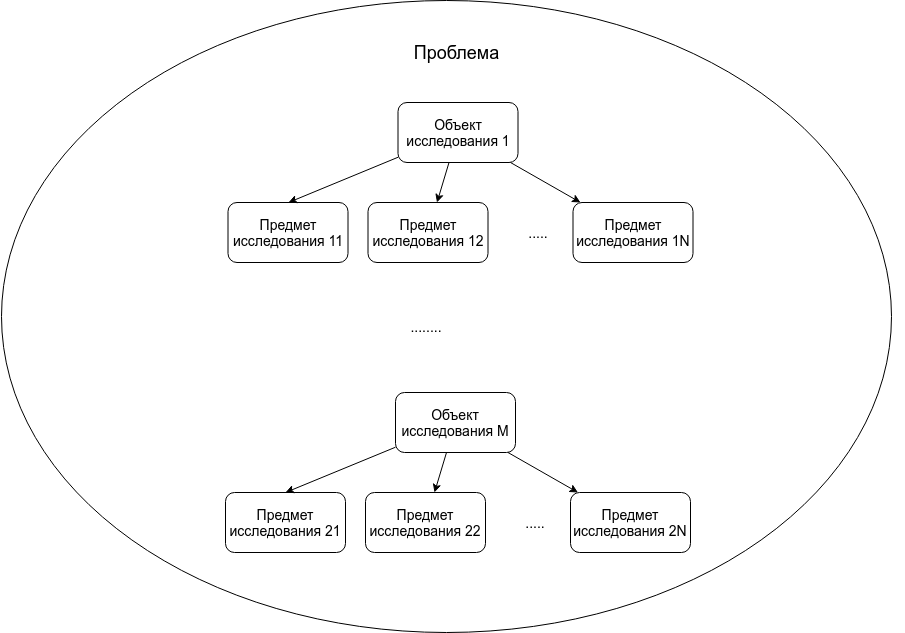
\includegraphics[width=13cm]{otnoshenie}
	%\caption{Иллюстрация процесса подготовки статьи.}
\end{figure}
В рамках ответов на ключевые вопросы, можно выстроить следующую иерархию с точки зрения убывания "широты постановки":

\begin{itemize}
	\item проблема,
	\item объект исследования,
	\item предмет исследования,
	\item цель,
	\item задачи.
\end{itemize}
При этом важно понимать, что в рамках одной проблемы всегда можно выделить более одного объекта исследования, у объекта исследования - множество свойств, а для пары "Объект, Предмет" - множество целей.

\subsection{Актуальность - технические приемы}
Ниже мы подобрали наиболее частые обоснования актуальности поставленной проблемы:

\begin{enumerate}
	\item Дать актуальную статистику
		\begin{enumerate}
			\item Вреда от проблемы ("ежегодно дикие слоны вытаптывают до миллиона гектаров ценной арктической тундры").
			\item Перспективности работы с проблемой ("стоимость рынка блёсен для слонов превысила 4 миллиарда долларов").
		\end{enumerate}
	\item Указать на пробелы в научном знании:
		\begin{enumerate}
			\item "На сегодняшний день не существует общепринятых теорий клёва слонов" (теоретический пробел).
			\item "Все зафиксированные эксперименты по ловле слонов сетью закончились трагическими неудачами" (экспериментальный пробел).
		\end{enumerate}
	\item Указать на неэффективность существующих решений ("существующие удочки не позволяют эффективно подсечь слона").
	\item Указать на перспективность направления, так как существуют исследования, связанные с данной областью ("ловля слонов является развитой отраслью научного знания. Наиболее важные результаты были получены в фундаментальных работах ...").
		\begin{enumerate}
			\item Перспективные выгоды от решения поставленной задачи (предложенный способ ловли молодых особей на мормышку способен существенно снизить травматизм хоботов) // Предложено пользователем Роман Иванов.
		\end{enumerate}
\end{enumerate}
Обратите внимание, что чем больше обоснований актуальности будет указано, тем лучше будет выглядеть ваша статья и тем более выгодное впечатление вы произведете как ученый.

Проблема – это одно предложение, которое характеризует очень широкую проблему, которую пытается частным образом решить ваша научная статья. Т.е., для выдуманной нашей статьи потенциальная проблема – потеря пакетов при их передаче дымовыми сигналами. Наша статья не может рассмотреть всеобщие варианты пакетов, трафика, погодных условий и т.п. Поэтому в статье будет рассмотрена неизбежный узкий кусочек проблемы, и статья попробует решить этот острый кусочек. Для ответа на этот ключевой вопрос мы должны сформулировать некое общее явление. Допустим, мы в статье отвечаем на вопрос, как улучшить качество связи при передачи пакетов в помощью дымовых сигналов для средней полосы России зимой в ясную погоду без ветра, используя березовые дрова как источник сигнала. Проблема у нас всегда будет шире.

Актуальность проблемы формулируется по следующей схеме:
\begin{itemize}
	\item первое предложение отвечает на вопрос, почему данную проблему необходимо решать;
	\item второе - почему она до сих пор не решена.
\end{itemize}

Почему проблему нужно решать? Здесь может быть множество разных аргументов. Для начинающих авторов является апелляция к статистикам, если это технические статьи. Если, например, мы рассматриваем выдуманную статью – есть проблема потери пакетов при передаче дымовыми сигналов. Мы апеллируем к статистике финансовых потерь от вот этого явления, этой проблемы. Как ухудшается в следствие этого трафик. Данные открыты, их можно найти в открытом доступе.

Другой способ обоснования необходимости решения проблемы – ее научная непроработанность. Развитие научного знания – хороший аргумент для обоснования актуальности. Ответом на второй вопрос о том, почему проблема еще не была решена, является описание трудностей, сопряженных с ее решением. Почему проблема является сложной. Для нашей выдуманной статьи сложностью является множество факторов, которые влияют на потери пакетов. Отсутствие мат. моделей, сложность существующих моделей, задающих динамику движения дыма в плотных слоях атмосферы в каких-то погодных условиях.

Собирая вместе научную проблему и актуальность, мы получаем формулировку научного противоречия. Научное противоречие построено по следующей схеме: проблема [такая-то] является важной и актуальной [актуальность], однако в данный момент она не решена, поскольку [почему].

Объект исследования представляет собой ту часть реального мира, которую мы исследуем в рамках нашей статьи. Предмет исследования -- свойства, связанные с объектом процессы и характеристики объекта исследования, которые мы непосредственно изучаем в рамках нашей работы. Одному объекту исследования может соответствовать несколько предметов.

Для нашей выдуманной статьи: объект исследования -- дымовые линии передачи данных, предмет исследования может быть различным -- защищенность от погодных помех, скорость передачи данных по дымовым линиям, алгоритмы маршрутизации пакетов на дымовых линиях.

Объект исследования достаточно подвижная вещь с точки зрения того, с какой точки зрения (технической науки) смотрите на проблему.

Например, передача сетевых пакетов с помощью дымовых сигналов смотрели как физики, то объектом мог быть дымовой след в атмосфере, а предмет -- оптические свойства дыма в атмосфере или его взаимодействие с атмосферными потоками воздуха.

Необходимо отметить, что в рамках одной проблемы может быть много разных объектов исследований. Поэтому, когда вы будете формулировать объект и предмет исследования, отталкивайтесь от тех результатов, которые у вас есть. Старайтесь в первую очередь определить те свойства и объекты, которые непосредственно у вас исследованы в ваших экспериментах или покрываются вашей моделью.

Цель и задачи научной статьи. Цель вашей работы – это одно предложение, которое формулирует желаемый результат. Задачи – это отдельные действия и компоненты, при выполнении которых ваша цель достигается. Как правило, каждая задача – это одно предложение. Важно про формулировку цели и задач понять следующее:

\begin{itemize}
	\item сумма задач должна определять цель (ни лишнего, ни через край);
	\item считается хорошим тоном, когда задачи повторяют условную структуру вашей работы. Не обязательно повторять названия разделов из задач, но    содержание должно быть отражено.
\end{itemize}

Самих задач не может быть очень много – это крупные блоки исследования.

Пример для нашей выдуманной статьи. Целью является исследование зависимости между потерей пакетов, передаваемых дымовыми сигналами, и направлением ветра. Задачи:

\begin{itemize}
	\item исследование существующих моделей передачи данных на подобных линиях
	\item связи, так и модели движения воздушных масс;
	\item учет направления ветра в новой модели помехозащищенности дымовых линий, проведение численных экспериментов, сопоставление численных экспериментов с натурными измерениями на реальных дымовых сигналах.
\end{itemize}

\subsection{Примеры определения объекта и предмета исследования}
Биологические науки
Объект исследования: популяция пингвинов.

Предметы:

динамика роста,
характер миграций,
агрессивность.
Технические науки
Объект исследования: методы распознавания и подсчета птиц на аэрофотоснимках.

Предметы:

качество распознавания,
скорость работы алгоритма,
работа алгоритма при ограниченных ресурсах.
Физико-математические науки
Объект исследования: математическая модель распознавания птиц.

Предметы:

сходимость,
точность,
устойчивость решений.

\subsection{Типовые ошибки при ответах на ключевые вопросы}

\subsubsection{Предмет и объект исследования}

\begin{enumerate}
	\item Предмет исследования не связан с объектом исследования.
	\item Слишком широкий объект исследования.
\end{enumerate}

\subsubsection{Проблема, цель и задачи}

\begin{enumerate}
	\item Поставлено более одной цели/проблемы, например, "Разработать метод оценки качества речи И оценить его эффективность"
	\item Проблема и/или цель имеют слишком узкую направленность/ уже чем фактическая цель работы - например “получить значение производительности библиотеки libxml” вместо “найти наиболее производительную библиотеку/ выработать метод оценки производительности”.
	\item Проблема формулируется как отсутствие чего-то, например, “отсутствие удобного/производительного/безопасного сервиса заказа такси”.  вместо “Организация удобного/производительного/безопасного сервиса заказа такси”.
	\item Проблема и цель явно не связаны.
	\item Задачи не раскрывают цель полностью.
\end{enumerate}


\subsubsection{Актуальность}

\begin{enumerate}
	\item Обоснования актуальности даны без ссылок на статистику и/или существующие работы.
	\item Обоснования сформулированы размыто, например "Ошибки деления на ноль приводят к значительным убыткам в вычислительных системах" вместо "В период с 2014 года ошибки деления на ноль привели к убыткам более 100 миллионов рублей". 
\end{enumerate}

\section{Обзор аналогов 1}
После ответов на ключевые вопросы нам необходимо провести обзор аналогов. Этот раздел может быть известен под названиями: обзор или анализ литературы, обзор существующих решений. Суть раздела – изучить существующие подходы к решению вашей проблемы, которая лежит в основе вашей будущей статьи и в деталях их исследовать. Это исследование проводится путем сравнения существующих решений и подходов по набору унифицированных критериев. После проведения этого сравнения, после характеристики по критериям формулируется некий вывод, который задает направление для дальнейшего исследования и позволяет спозиционировать то, что вы делаете, относительно работ других ученых. Структурно обзор состоит из следующих подразделов:

\begin{itemize}
	\item описание принципов отбора альтернатив или существующих подходов, аналогов, потенциальных решений проблемы;
	\item описание подобранных альтернатив;
	\item описание критериев, по которым вы будете характеризовать альтернативы;
	\item сравнение альтернатив по критериям и их характеристики – часто в виде таблицы для наглядного сопоставления;
	\item выводы о том, каким путем надо пойти, чтобы решить поставленную проблему.
\end{itemize}

Данный раздел задает тон всей статье. Поэтому все эти подразделы должны быть обоснованы, должны иметь в тексте прямое обоснование, которое говорит, почему именно так подбирали аналоги, почему именно эти альтернативы были выбраны. Для обоснования рекомендую очень сильно привязываться к ответам на ваши ключевые вопросы, которые дадут вам правильное направление для формулирования подбора и сравнения аналогов.

\subsubsection{Структура обзора}
\begin{itemize}
	\item Описание принципа отбора аналогов.
	\item Характеристика и перечисление отобранных альтернатив.
	\item Список критериев с обоснованием выбора каждого.
	\item Характеристика каждой альтернативы по каждому критерию.
	\item Таблица сравнения (строки - аналоги, столбцы критерии).
	\item Выводы.
\end{itemize}

Основные проблемы начинающих авторов начинаются именно на этапе поиска аналогов, альтернативных решений.

Главная проблема – отсутствие аналогов. Часто начинающий автор выполняет поиск по точному названию исследуемой им области науки – ищет алгоритмы, в статьях, научных работах и не находит в конкретно такой формулировке, как поставлена задача. И автор в своей работе пишет, что аналогов нет. Такое утверждение в корне неверно, не будет упрощением считать, что в 99\% случаев аналоги есть, они есть практически всегда. Редакторы при проверке статей зачастую воспринимают это как красную тряпку. Это одно из самых простых замечаний, которые даже начинающие рецензенты и редакторы видят.

Для того чтобы найти аналоги, мы предлагаем вам взглянуть на проблему немного по другому. Давайте считать, что аналогом является любой способ решения нашей проблемы, каким бы он не был странным или непохожим на то, что мы рассматриваем в качестве целей нашей работы. Это означает, что мы не должны ограничивать рассмотрение аналогов только тем конкретным типом систем, которые мы собираемся изобрести. Мы должны рассматривать родственные системы, системы, которые построены по другим принципам, но исполняют тоже функциональное назначение. Мы должны рассматривать естественных конкурентов решения проблем. Например, если речь идет про алгоритмы, мы должны рассматривать их эмпирические аналоги – эвристики, которые могут применяться активно в производстве, в различных видах деятельности и давать неплохие результаты. Все, что конкурирует с нами за решение проблемы, все что помогает ее решить, все, что позволяет к ней подобраться – является аналогом.

Чтобы сделать всеобъемлющий обзор аналогов, выполнить поиск, чтобы альтернативные решения проблемы были найдены. Основной принцип – необходимо увеличивать широту взгляда на проблему в процессе обзора аналогов.

Давайте в качестве примера считать, что объектом обзора являются нейросетевые алгоритмы прогнозирования спроса и мы предлагаем свой алгоритм для прогнозирования спроса и должны исследовать, как обстоит ситуация с подобными решениями. У нас есть термин, который состоит из понятий – “нейросетевой”, “алгоритм”, “прогнозирование”, “спрос”. Для всеобъемлющего поиска аналогов, мы должны свериться со словарями, учебниками и энциклопедиями, и понять, какие определения соответствуют отдельным терминам нашего объекта. Что такое “спрос”, “нейронная сеть”, “прогнозирование”, “алгоритм”, “алгоритм прогнозирования”, “нейросетевое прогнозирование”. Мы должны рассмотреть все определения и выписать их отдельно. Это может показаться странным или очевидным. Возможно, автор уже знает, что это такое. Но на самом деле в ней есть глубокий смысл – очень часто в научных статьях описываются альтернативы тому, что мы хотим сделать – алгоритм прогнозирования спроса – но они могут описываться другими словами с использованием альтернативными, похожими, созвучными терминами. Поэтому, для каждого компонента нашего объекта мы должны понять, есть ли какие-нибудь синонимы для этого термина, похожие, созвучные, обладающие схожим смыслом. К какому классу и надсистеме он относится? Если мы хотим получить всеобъемлющий обзор, желательно получить правильный, каноничный перевод на английский язык, чтобы рассмотреть иностранные источники. Например, у нас есть “спрос” – канонический показатель, функция, это его надсистема. Какими-то просторечными синонимами могут быть “доходность”, “выручка” и т.д. Это разные понятия, но находятся по смыслу рядом. Перевод “спрос” взять из словаря. Аналогично можем поступить с “алгоритмом” и “нейронными сетями”. Нейронная сеть представляет собой аппроксиматор, синонимы могут быть только однокоренные “нейронная сеть”, “сеть Кохонена”, “персептрон”, “обратное распространение ошибки”, которые про нейронную сеть. Надсистема – аппроксиматоры, т.к. НС работает как аппроксиматор. Для алгоритма синонимом может быть: последовательность, метод, методика, способ, технология. Эти понятия не тождественны, но они в общем смысле об одном и том же – это все про последовательности действий. Мы с вами имеем облако синонимов. Что необходимо делать дальше? Во-первых, поискать аналоги по прямому совпадению: “НС алгоритмы прогнозирования спроса”. Допустим, не нашли. Дальше мы должны опускать отдельные компоненты определения и искать по его подмножествам, например, “алгоритмы прогнозирования спроса” или “нейросетевое прогнозирование спроса”. Если по ним ничего не находим, то спускаемся на уровень ниже и рассматриваем абстрактные модели: модели спроса, модели НС, типы НС, виды НС, методы и спросы прогнозирования и уже можем их использовать в качестве аналогов с точки зрения их применимости для наших задач. Тогда наше сравнение будет: мы сравниваем предлагаемые алгоритмы и системы с точки зрения пригодности. У нас есть эконом. модель спроса, нейронная сеть, которая умеет прогнозировать спрос, есть вычислительная модель спроса (разностная схема) – собираем все в таблицу, выделяем критерии и сравниваем, как с помощью этих решений можно решить нашу задачу. Не стоит забывать, что мы выделили класс и надсистему для каждого из понятий. Параллельно нужно проводить поиск по родственным понятиям и соседним классам этих подсистем. Например, мы не нашли нейросетвых алгоритмов прогнозирования спроса, мы можем поискать нейросетевые алгоритмы прогнозирования убытков и других экономических показателей, мы можем повторить эту операцию для каждого экономического показателя, для разных видов аппроксиматоров, например, не только прогнозирования, но и для принятия решений в области экономических действий. Мы получаем очень большое дерево вариантов, куда можно наложить английский язык и дерево станет еще больше. Если внимательно поискать по каждой фразе, которая получается таким алгоритмом статьи, то сколько-то аналогов найти получится. Идя таким путям от частных формулировок к более абстрактным, сворачивая в различные виды систем и в соседние классы, мы получим большой обзор, если каждую из найденных альтернатив проработать. Сам этот обзор уже будет иметь большую ценность, если будет описаться на релевантные источники научных данных.

\subsubsection{Алгоритм поиска аналогов}
Предлагаемый алгоритм является максимально общим, и представляет собой попытку собрать всевозможные способы найти аналогичные и альтернативные способы решения проблемы вашего исследования. В определенных отраслях науки и техники отдельные этапы алгоритма могут оказаться лишними, например поиск тривиальных и эмпирических решений для теоретической статьи.
\paragraph{0. Предварительная подготовка}
Предположим, что вы пишите статью и вам необходимо найти существующие методы решения проблемы. Также будем считать, что у вас есть ответы на ключевые вопросы.
\paragraph{1. Поиск максимально похожих аналогов}
\begin{enumerate}
	\item Сформулируйте одним предложением общее название для типа систем, которые вам интересны (например "Нейросетевые алгоритмы прогнозирования спроса").
	\item Сформулируйте перевод полученного названия на английский язык, используя устоявшиеся термины.
	\item Выполните поиск по названию на русском и английском, изучите статьи, зафиксируйте найденные аналоги.
\end{enumerate}
\paragraph{2. Поиск по неполному совпадению}
\begin{enumerate}
	\item Разделите название на всевозможные отдельные понятия (например: нейросети, нейросетевые алгоритмы, алгоритмы, алгоритмы прогнозирования, нейросетевое прогнозирование, прогнозирование спроса ....).
	\item Сформулируйте переводы на английский для полученных "подназваний".
	\item Выполните поиск и зафиксируйте те, результаты, которые можно использовать в качестве решения вашей проблемы.
\end{enumerate}

\paragraph{3. Поиск смежных систем}
\begin{enumerate}
	\item Определите, какие смежные типы систем / моделей для найденных в п. 2 "подназваний" (например, вместо нейросетевых алгоритмов прогнозирования можно рассмотреть байесовский подход, нечеткую логику и т.д.).
	\item Сформулируйте переводы на английский.
	\item Выполните поиск и зафиксируйте те, результаты, которые можно использовать в качестве решения вашей проблемы.
\end{enumerate}

\paragraph{4. Поиск тривиальных и эвристических решений}
Ответьте на следующие вопросы:
\begin{enumerate}
	\item К чему приводит отсутствие решения и как это выражается количественно?
	\item Может ли проблема решиться без внешнего вмешательства?
	\item Существуют ли не технологичные (не научные) решения вашей проблемы?
	\item Какие эвристики применяются в решении рассматриваемой проблемы?
\end{enumerate}
Сформулируйте подходы к решению проблемы из ответов - это будут наивные и эвристические решения.

\paragraph{5. Базовые формализмы}
\begin{enumerate}
	\item Опираясь на п. 2, определите, какие базовые формализмы (модели, законы и закономерности ) лежат в основе "подназваний".
		\begin{enumerate}
			\item Можно ли его использовать в качестве решения проблемы (напрямую) или в качестве вспомогательного инструмента (косвенно)?
			\item Насколько популярным и общепринятым является использование формализма в аналогичных исследованиях?
		\end{enumerate}
	\item Для каждого из базовых формализмов ответьте на вопросы:
	\item Формализмы, которые можно использовать для решения проблемы, можно выделить в качестве средств для реализации альтернативных решений проблемы.
\end{enumerate}

\subsubsection{Пример (неполный) поиска аналогов}

\begin{figure}[H]
	\centering
	
\includegraphics[width=15cm]{analogs_pyramid}
	%\caption{Иллюстрация процесса подготовки статьи.}
\end{figure}
Что можно еще упомянуть в качестве базовых моделей / формализмов:

\begin{itemize}
	\item любые мат.модели в экономике,
	\item модели выручки / прибыли и других экономических параметров,
\end{itemize}

Варианты эвристик:

\begin{itemize}
	\item считать, что спрос зависит только от дня недели / времени года / месяца;
	\item считать, что спрос сегодня это среднее от показателей двух последних дней.
\end{itemize}

Варианты наивных решений:

\begin{itemize}
	\item считать, что спрос имеет постоянное значение;
	\item считать, что спрос возрастает с постоянной скоростью.
\end{itemize}
Отсутствие решения - вести торговлю без использования какого-либо прогноза.

\subsubsection{Коды научной классификации}
Дополнительным способом найти аналоги является использование кодов научной классификации. Данные системы структурируют отрасли научного знания с помощью иерархических численно-буквенных обозначений.

Примерами таких систем являются (по ссылкам даны каталоги кодов):
\begin{itemize}
	\item Универсальная десятичная классификация.
	\item Государственный рубрикатор научно-технической информации.
	\item Коды международной классификации (OECD).
\end{itemize}
Как же данные системы помогут вам найти аналоги?

\begin{itemize}
	\item Определите номер(а) вашей отрасли науки в каждой из систем кодов научной классификации.
	\item Используйте полученные номера в системах поиска статей.
\end{itemize}





\section{Обзор аналогов 2}
\section{План-проспект}
\section{Основыне и дополнительные материалы}

\end{document}


 
